% A template for MCM contest solution
% Make sure 'reedmcm.cls' and 'mcm.sty' are in the directory that you're running latex from.
% These are meant to be used with pdflatex.
% Note: natbib for bibliography.
\documentclass[12pt]{reedmcm}
\usepackage{mcm}
\graphicspath{{./images/}}

%Title
\title{\textbf{Title of the Solution}}
\team{22555} % Put your team control number here. No actual names!
\contest{MCM}
\question{A} % Problem A or B?
\date{\today}

%Headers
\usepackage{fancyhdr}
\pagestyle{myheadings}
\setlength{\headheight}{13.6pt}
\setlength{\headsep}{20pt}
\pagestyle{fancy}
%%% Redefine the plain pagestyle so that it includes the ``page x of
%%% y'' information, as well.
\fancypagestyle{plain}{%
  \fancyhf{} % clear all header and footer fields
  \fancyhead[LO,RE]{Team \# 22555}
  \fancyhead[RO,LE]{Page~\thepage\ of \pageref{LastPage}}
  \fancyfoot[c]{\thepage}
  \renewcommand{\headrulewidth}{0pt}
  \renewcommand{\footrulewidth}{0pt}
}
%%% Define the header as per the contest regulations.
\fancyhead{}
\fancyhead[LO,RE]{Team \# 22555}
\fancyhead[RO,LE]{Page~\thepage\ of \pageref{LastPage}}


\begin{document}

% The Summary of your solution must be on the first page.
%  The contest rules specify that you should include a one-page summary of your report. 
%  You want a brief restatement of the problem followed by a largely \emph{non-technical} description of what you've done.
%  Try to avoid using mathematical notation.
%  You probably want to write a few paragraphs, around half to two-thirds of a page.
%  From COMAP: 
%  "The summary is a very important part of your MCM paper. The
%    judges place considerable weight on the summary, and winning
%    papers are sometimes distinguished from other papers based on
%    the quality of the summary. To write a good summary, imagine
%    that a reader may choose whether to read the body of the paper
%    based on your summary. Thus, a summary should clearly describe
%    your approach to the problem and, most prominently, what your
%    most important conclusions were. The summary should inspire a
%    reader to learn the details of your work.  Your concise
%    presentation of the summary should inspire a reader to learn
%    the details of your work. Summaries that are mere restatements
%    of the contest problem, or are a cut-and-paste boilerplate
%    from the Introduction are generally considered to be
%    weak."

\begin{summary}
  Genetic algorithm determines the shape that is most suitable for even heat distribution.
  The heat distribution on the pan and brownie is computed by the diffusion equation.
  We solve the diffusion equation numerically in general using the finite-difference method.
  We also solve the diffusion equation analytically for a special case to verify our numerical solution.
  Chaotic transformations, Arnold's Cat map and Chirikov Standard map, produces random shapes.


  \end{summary}
  % End of Summary

% After the Summary, the actual solution starts.
\maketitle
\tableofcontents
\listoffigures
% \listoftables  

\section{Introduction}
SciPy to simulate the heat equation.
Restatement Clarification of the Problem: state in your own words what you are going to do.

It should include a restatement of the problem, the history and context of the problem, and your work and results.
Mention the traditional methods that are used to solve the particular kind of problems.

\subsection{Approach}
Flow chart

\section{The Model}
\subsection{Assumptions and Justifications}
\begin{itemize}
  \item The temperature of the oven is kept constant at $T$.
   The oven is preheated before the brownie and pan are placed inside.
   Our model is agnostic about the size or shape of the model.

  \item We test a pan one at a time. 
    Even in the case where more than one pans is placed in the oven, our model is valid as long as the surface of each pan is kept at a constant temperature.

  \item We assume that pan's walls are flat surfaces. While it is possible to consider walls that are curvilinear, we will assume this for the simplicity of the model.
\end{itemize}

\subsection{Variables and Constants}
\begin{itemize}
  \item $n\times m$: grid size
  \item $H$: pan's wall height
  \item $\alpha$: pan's wall slope
  \item $A$: pan's area
  \item $T_{oven}$: the oven's internal temperature
  \item $T_{room}$: the room temparature
  \item $Fit_{pack}$: the fitness of the shape of a pan measured by the number of the same shapes that can be packed in a oven
  \item $Fit_{heat}$: the fitness of the shape of a pan measured by how evenly heat is distributed over the pan
  \item $K_{pan}$: the conductivity constant of the pan
  \item $K_{br}$: the conductivity constant of the brownie
\end{itemize}

\subsection{Goal}
\begin{itemize}
  \item Determine the optimal wall shape in terms of the distribution of heat.
  \item Determine the optimal base shape in terms of the distribution of heat.
  \item Determine the optimal base shape in terms of the number of pans that can fit in the oven.
\end{itemize}

\section{The Baking Simulation}
\subsection{The Diffusion Equation}
\subsection{Parameter Fitting}

\section{Shapes}
\subsection{Assumptions on Shapes}
\begin{enumerate}
  \item The area is fixed to $A$. To determine the optimal shape, we use $A=1$. The effects of varying $A$ is explored separately.
\end{enumerate}

\subsection{Mutation, Area-Preserving Map, and Chaos}
In GA, mutation serves as a means of introducing new kinds of shapes that are potentially successful.
Since our goal is to compare different shapes with fixed area, we need to mutate shapes in a way such that does not alter the area.
Thus, mutation of shapes naturally require \textit{area-preserving map}.
Area-preserving map is a measure-preserving map in a two-dimensional sense, i.e. $m(L^{-1}) = m(L)$, where $m$ is the Lebesgue measure.
For example, suppose $L$ is a linear transformation.
If $\det(L) = 1$ then it is an area-preserving map; the class of such maps correspond to the special linear group $SP(2,R)$.
A typical member of $SP(2,R)$, however, does not bring about a radical change to a shape.
For example, the matrix
\begin{equation*}
\begin{pmatrix}
    \cos\theta & -\sin\theta  \\
    \sin\theta & \cos\theta  
  \end{pmatrix}
\end{equation*}
as a linear map corresponds to the rotation by $\theta$. 
Although this characteristic is suitable as a way of introducing slight modifications to a pre-existing shape, applications of such maps would not create an entirely new shape.
The observation motivates us to employ chaotic maps instead.
We can think of chaotic maps as having a higher mutation rate than non-chaotic maps.
Hence, we can use chaotic maps as a way of creating a random shape, which would correspond to generating a random rational number in a usual GA.
Mutations of shapes by area-preserving chaotic maps allow our GA to explore the solution space that would not be easily accessible by non-chaotic transformations.
In particular, we employ two chaotic maps: the \textbf{cat map} and \textbf{kick map}.

\subsection{The Cat Map}
We use the cat map (commonly refered to as the "Arnold's Cat Map") to mutate shapes.
Arnold's cat map is a chaotic, area-preserving map on a two-dimensional torus \citep{hilborn}.
The cat map $F$is defined as
\begin{equation*}
  F: (x,y) \mapsto (2x + y, x + y) \mbox{ (mod 1)}.
\end{equation*}
The corresponding matrix is
\begin{equation*}
A =
\begin{pmatrix}
    2 & 1  \\
    1 & 1  
  \end{pmatrix},
\end{equation*}
and clearly, $\det(A) = 1$.
In order to obtain a wider variety of shapes, we parametrize the Arnold's map as follows:
\begin{equation*}
  F: (x,y) \mapsto (kx + (k-1)y, x + y) \mbox{ (mod 1)},
\end{equation*}
where $k \in \mathbb{R}$, $0 \leq k \leq 5$.
Note that the determinant of the corresponding matrix
\begin{equation*}
\begin{pmatrix}
    k & k-1  \\
    1 & 1  
  \end{pmatrix}
\end{equation*}
is one.
Therefore, the parametrized Arnold's map is area-preserving.
\begin{figure}[t]
  \centering
  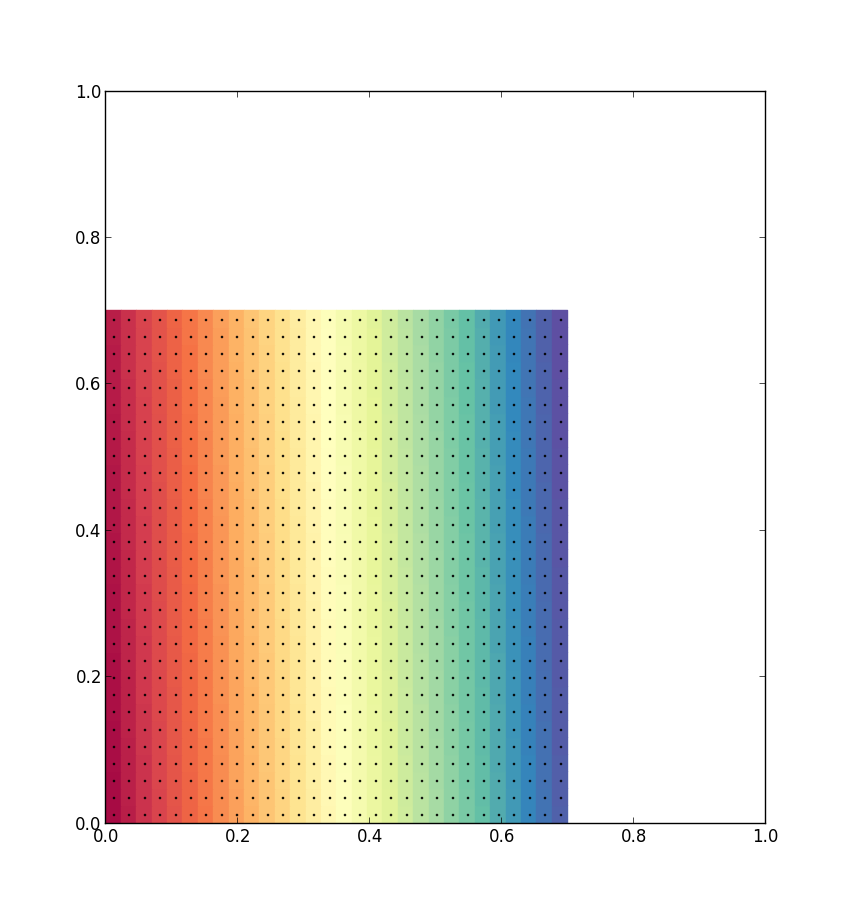
\includegraphics[width=0.6\textwidth]{square_049_900}
  \caption{A square $A = 0.49$ (i.e. the length of each edge is 0.7). Each square consists of patches. This square, for instance, consists of 400 patches, each represented with different colors.}
  \label{fig:square}
\end{figure}
The cat map stretches and folds the domain, and as a result, it produces thin strips.
The parameter $k$ determines the thickness of the strips.
The higher the value of $k$, the thinner the strips are (Fig.~\ref{fig:catmap_demo1}).
\begin{figure}[t]
  \centering
  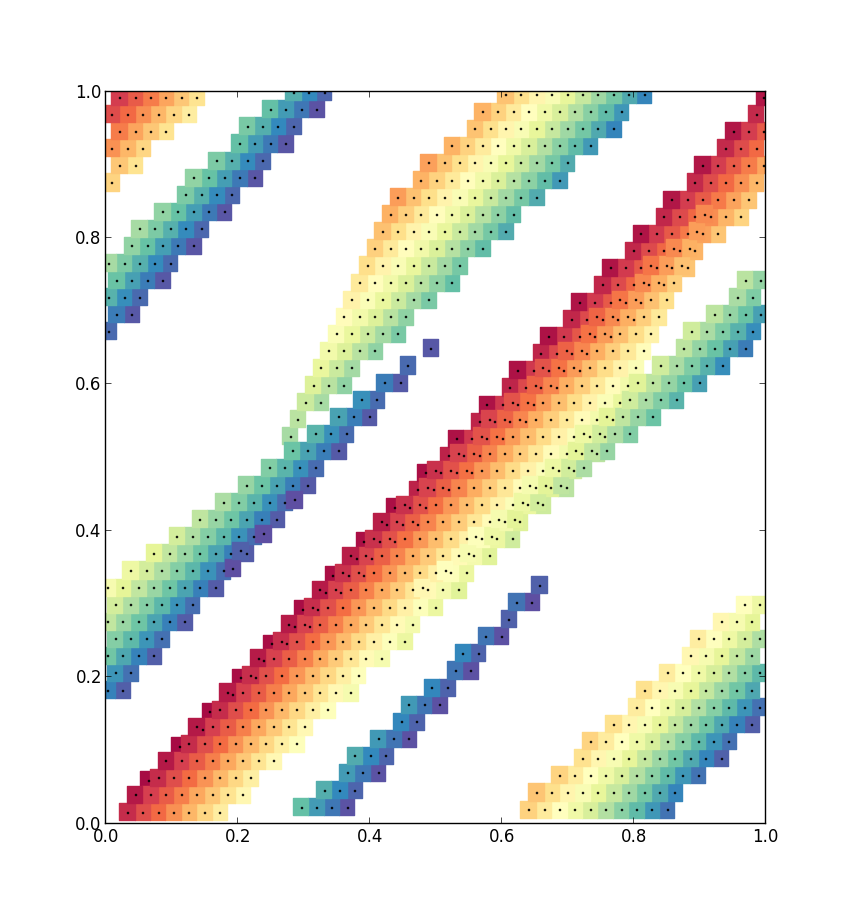
\includegraphics[width=0.4\textwidth]{catmap_1-5}
  \hspace{2cm}
  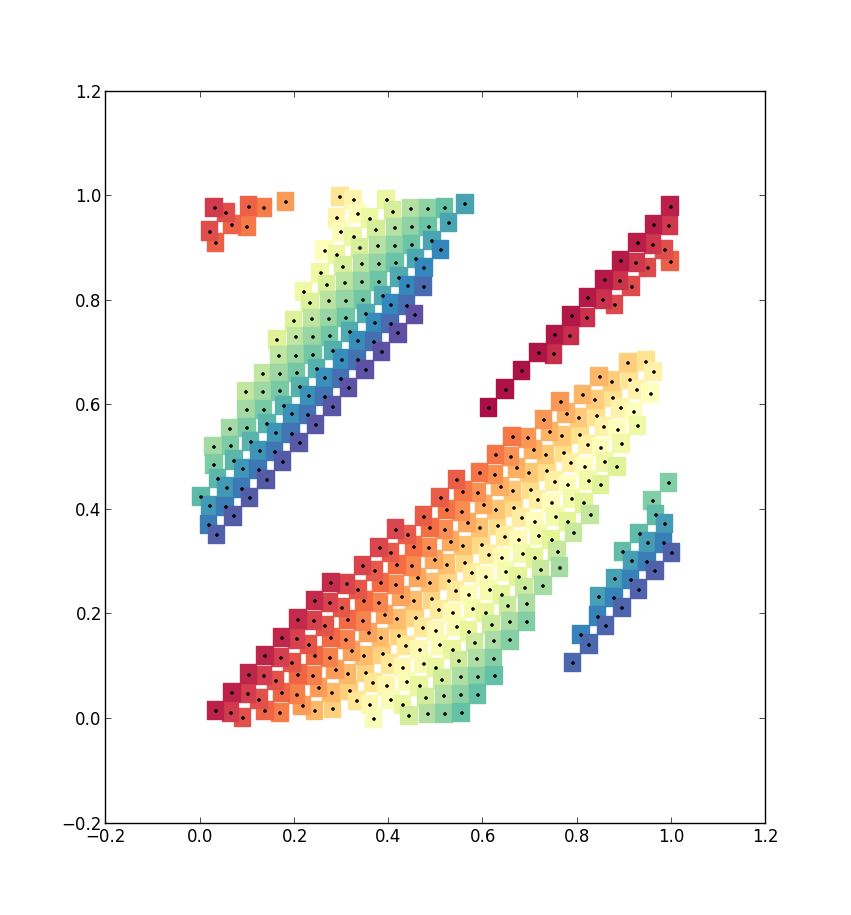
\includegraphics[width=0.4\textwidth]{catmap_3}
  \caption{Cat Map. left: $k=1.5$; right: $k = 3$. After one iteration. 
    Colors of the patches correspond to those in (Fig.~\ref{fig:square}).
    The one with greater $k$ tends to stretch the square to the $x$-direction, and splits the square region into thinner strips.
  }
  \label{fig:catmap_demo1}
\end{figure}

Although, $k$ can be any real number, parameters $k_0$ and its negative $-k_0$ result in effectively the same transformation, since the mapped images would be symmetric about the origin, and we take modulus 1 of the points.
Thus, we can only use $k \in \mathbb{R}^+$ without losing shapes in the solution space.
Also, the cat map would tend to stretch the unit square to the $x$-direction for greater $k$.
We will use $k \leq 10$, because, in a simulation using a limited precision, $k\geq 10$ does not give rise to appreciably different shapes (Fig.~\ref{fig:catmap_demo2}).

\begin{figure}[t]
  \centering
  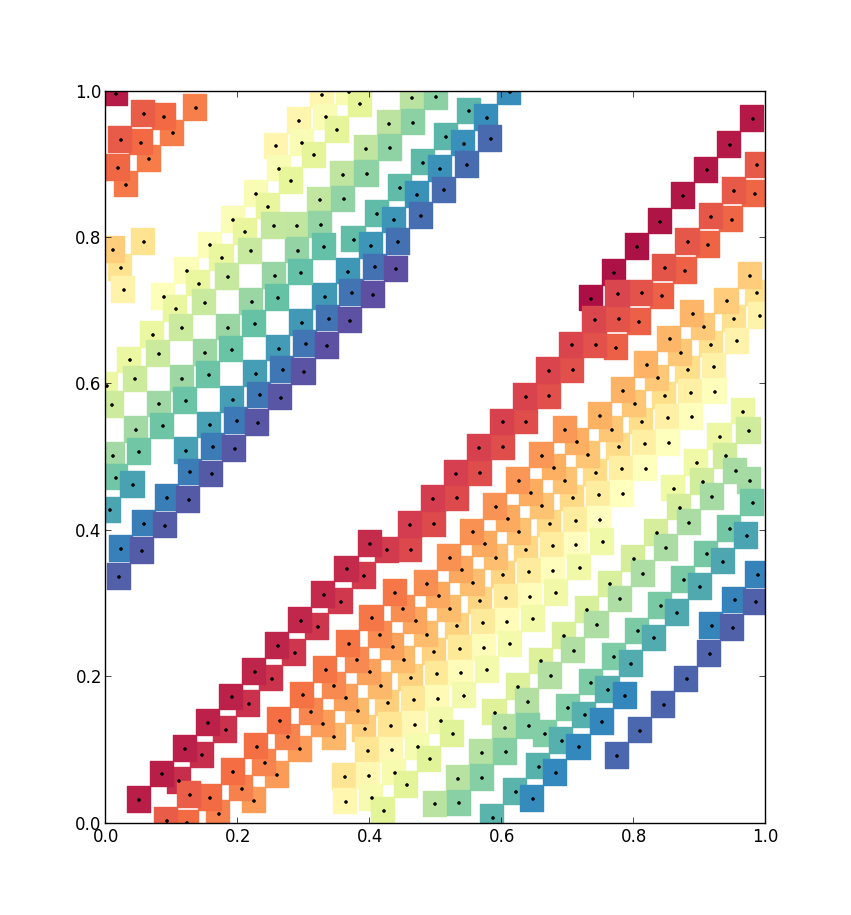
\includegraphics[width=0.4\textwidth]{catmap_10}
  \hspace{2cm}
  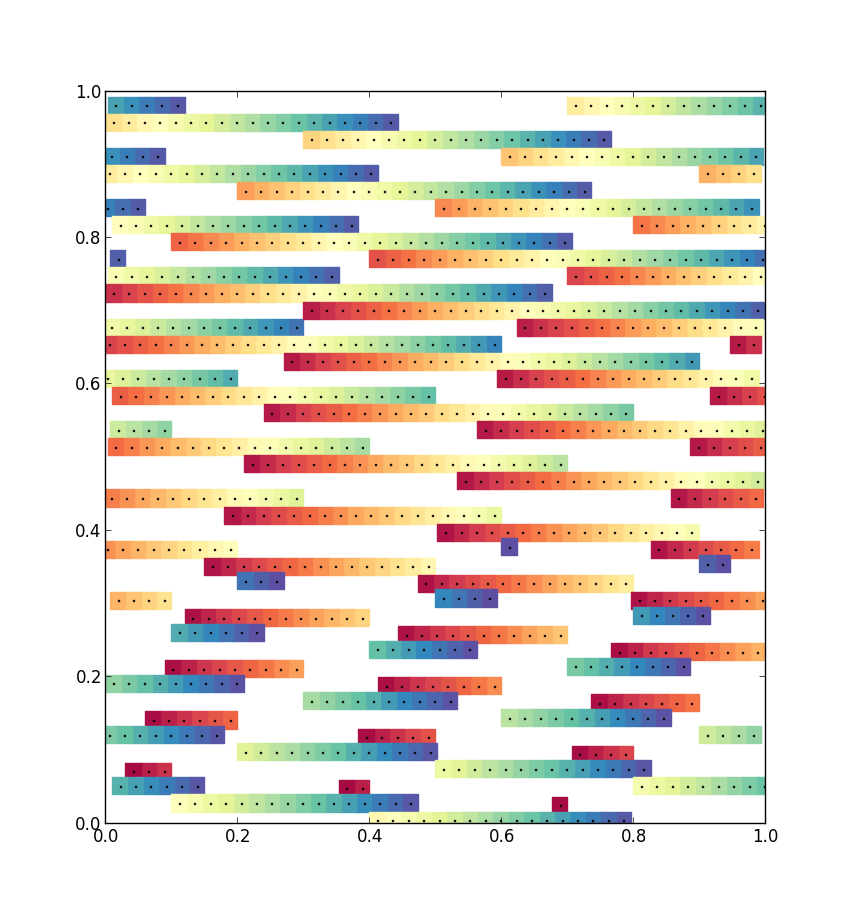
\includegraphics[width=0.4\textwidth]{catmap_30}
  \caption{Cat Map. left: $k=10$; right: $k = 30$. After one iteration. 
    Although the two images are not exactly the same, the differences seem not to be significant from a qualitative point of view.
  }
  \label{fig:catmap_demo2}
\end{figure}

\subsection{The Kick Map}
The other area-preserving chaotic map that we employ, the \textit{kick map}, is usually called the Chirikov's Standard Map \citep{ott}.
Qualitatively, the kick map \textit{swirls} a shape, a complementary action of the cat map, which stretches a shape into thin strips.
The kick map is defined as:
\begin{align*}
  y &\mapsto y + k \sin x \mbox{ (mod $2\pi$)} \\
  x &\mapsto x + y \mbox{ (mod $2\pi$)},
\end{align*}
where updates of $y$ and $x$ are done asyncronously ($y$ first).
The effects of the cat map is stronger for higher value of $k$ (Fig.~\ref{fig:kickmap_demo1}).
%
\begin{figure}[t]
  \centering
  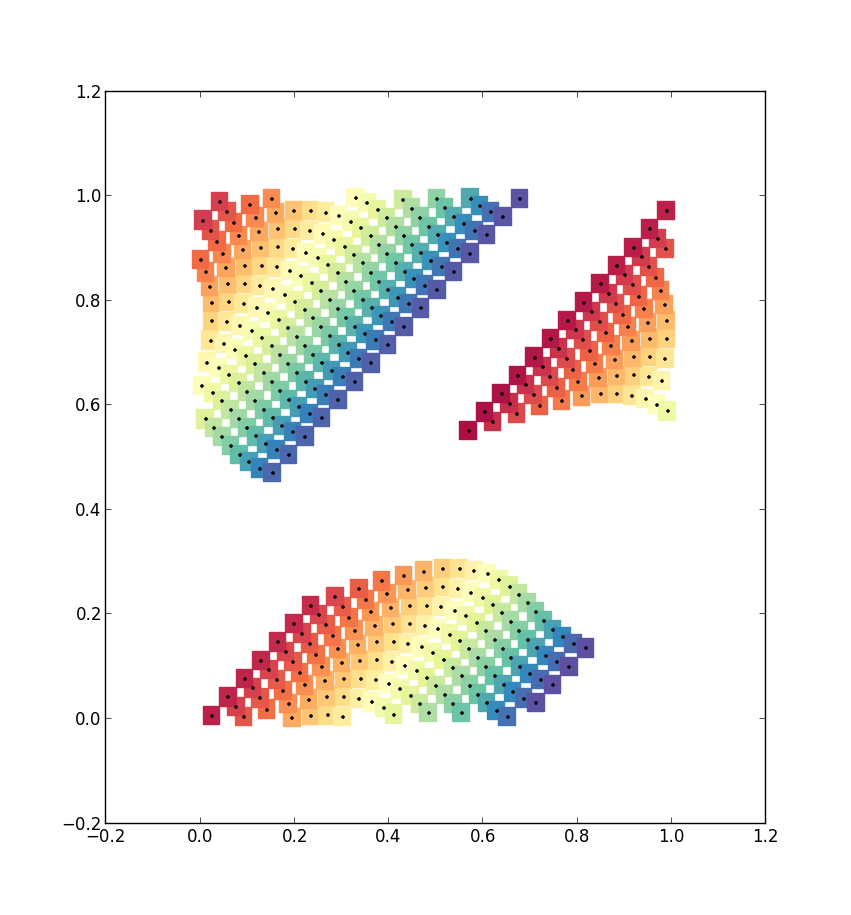
\includegraphics[width=0.4\textwidth]{kickmap_05}
  \hspace{2cm}
  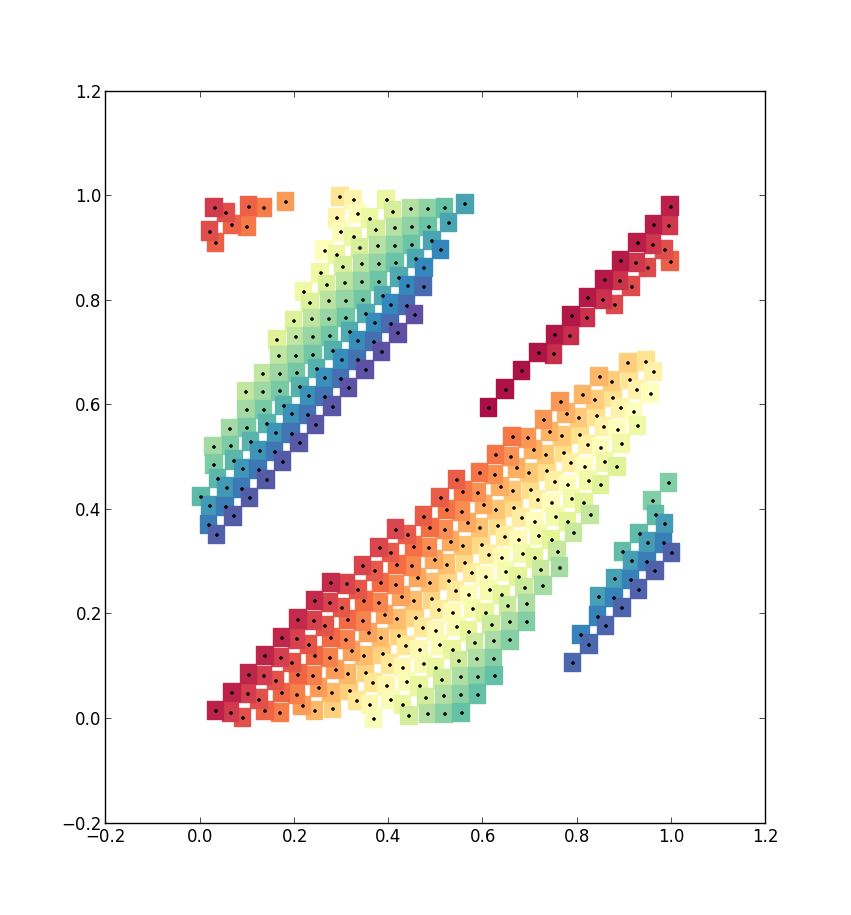
\includegraphics[width=0.4\textwidth]{kickmap_3}
  \caption{The kick map. left: $k=0.5$; right: $k = 3$. After one iteration. 
    The kick map with a higher value of $k$ has stronger effects on the domain.
  }
  \label{fig:kickmap_demo1}
\end{figure}
%
As $k$ approaches $1$, the kick map becomes more and more chaotic.
It is known that the chaotic border is 0.971635... \citep{spedia}.

\begin{figure}[t]
  \centering
  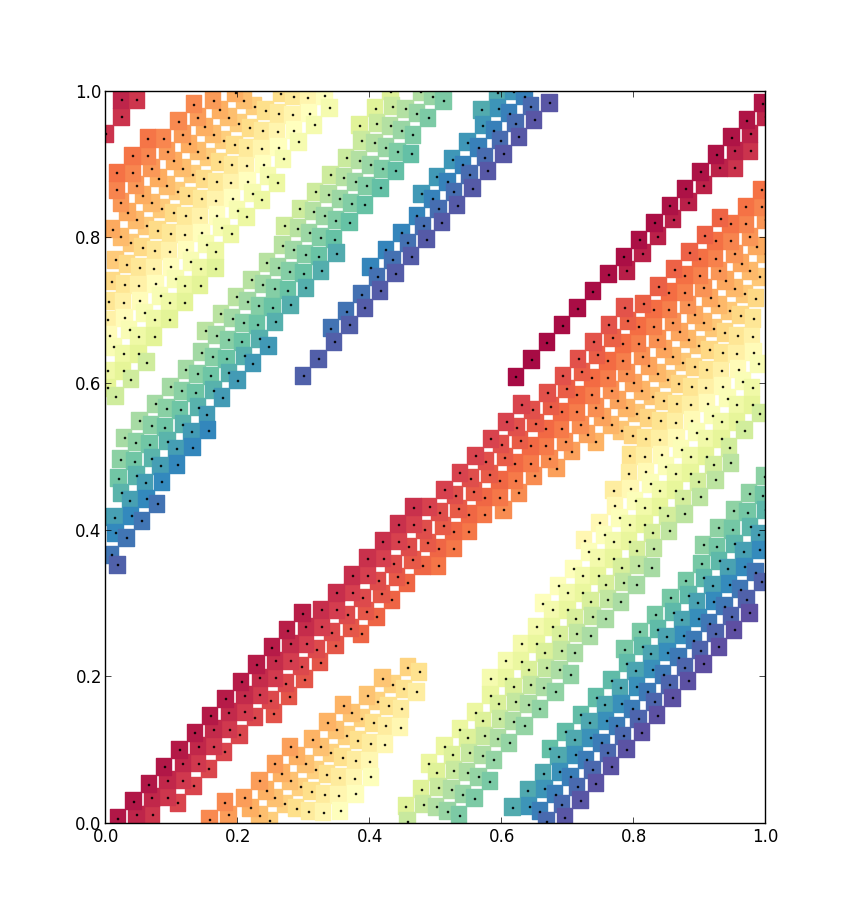
\includegraphics[width=0.4\textwidth]{kickmap_2pi}
  \hspace{2cm}
  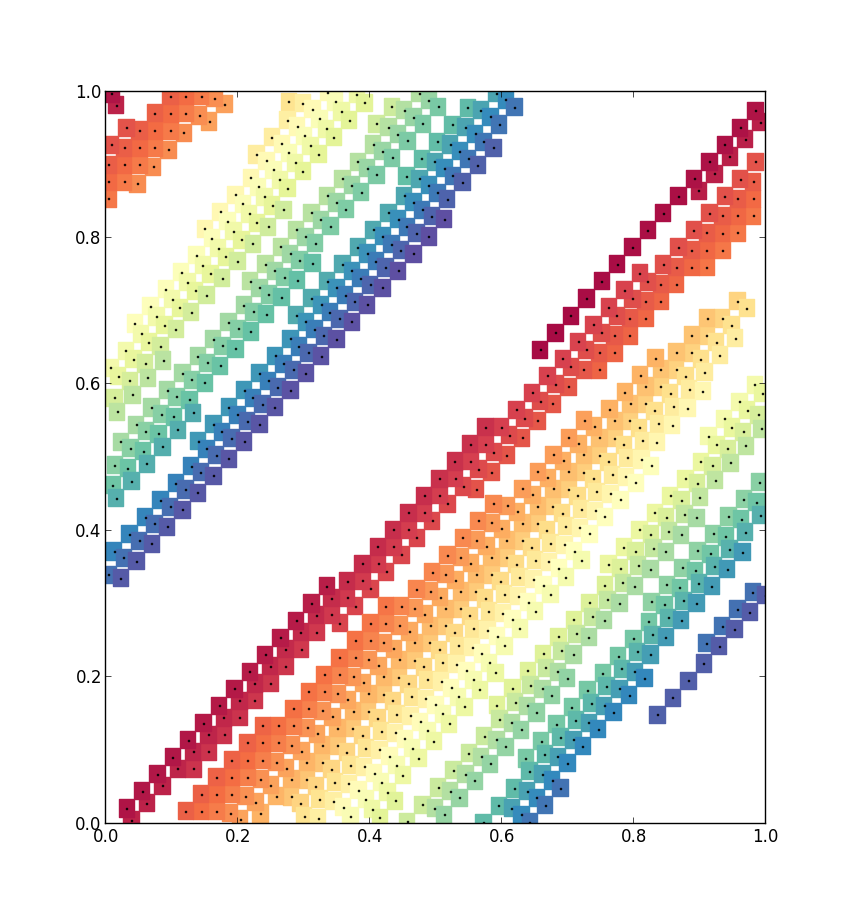
\includegraphics[width=0.4\textwidth]{kickmap_3pi}
  \caption{The kick map. left: $k=10$; right: $k = 30$. After one iteration. 
    Although the two images are not exactly the same, the differences seem not to be significant.
  }
  \label{fig:kickmap_demo2}
\end{figure}

Although we would like to apply the kick map to the unit square, the original kick map is a function from $[0,2\pi] \times [0,2\pi]$ to the same region.
We use the following version of the kick map whose domain and image are the unit square:
\begin{align*}
  y &\mapsto \frac{\pi + 2\pi y + k \sin (2\pi x)}{2\pi} \mbox{ (mod 1)}\\
  x &\mapsto \frac{2\pi (x + y)}{2\pi} \mbox{ (mod 1)}.
\end{align*}
In plain words, the coordinates of each point in the unit square is scaled by $2\pi$ prior to the application of the original kick map, then scale the result by $1/2\pi$.
Taking into account of the chaotic border ($k\approx 1$ in the original kick map), we take the range of $k$ to be $(0,2\pi)$.

\subsection{Generation of Random Shapes}
Iterate the unit square (Fig.~\ref{fig:square}) $0 \leq k \leq 10$ and $0 \leq k \leq 2\pi$.
In many cases, random iterations result in a chaotic shape that is apparently not suitable as a shape for the pan. 
However, the process may obtain orderly shapes such as those in Fig.~\ref{fig:order}.
\begin{figure}[t]
  \centering
  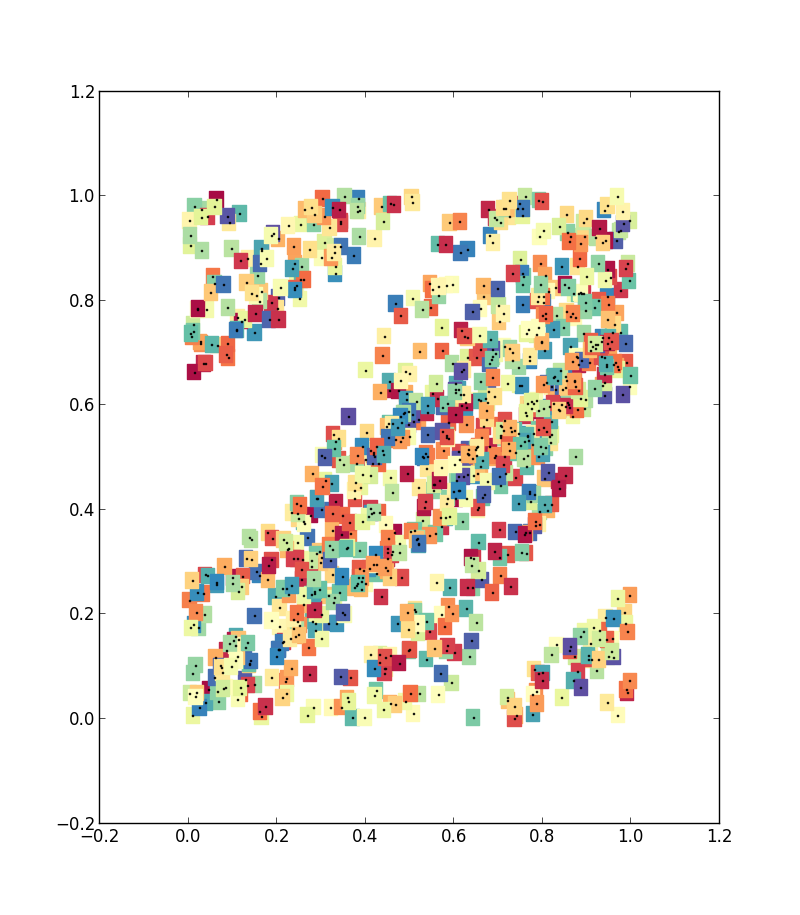
\includegraphics[width=0.4\textwidth]{random2}
  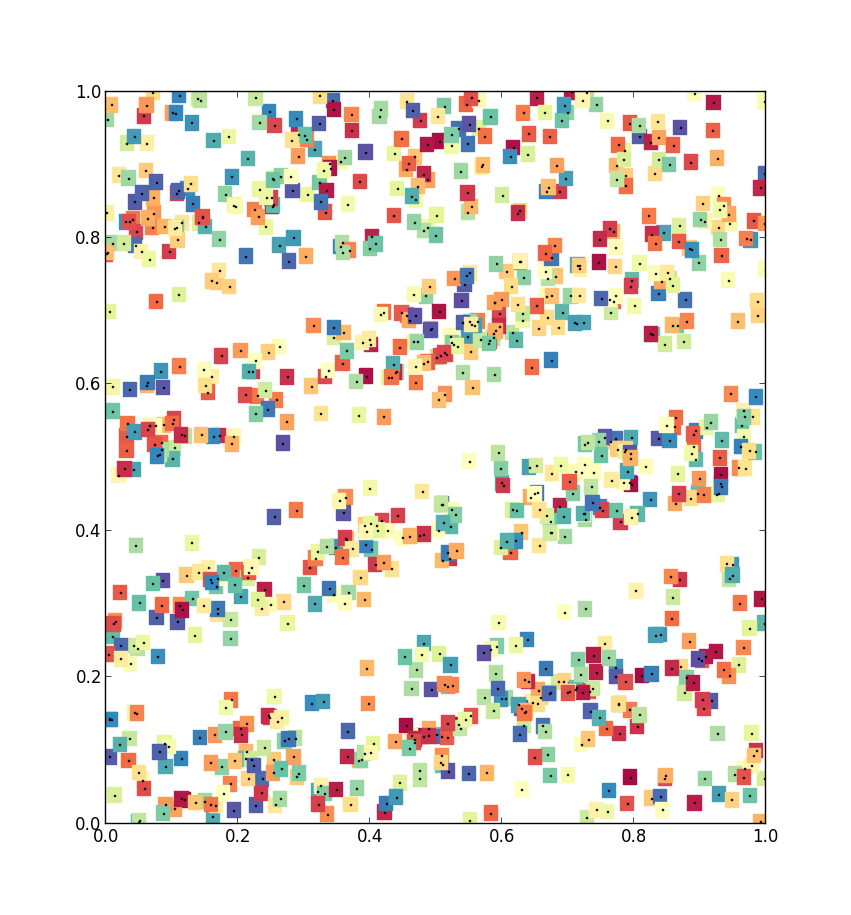
\includegraphics[width=0.4\textwidth]{random128}
  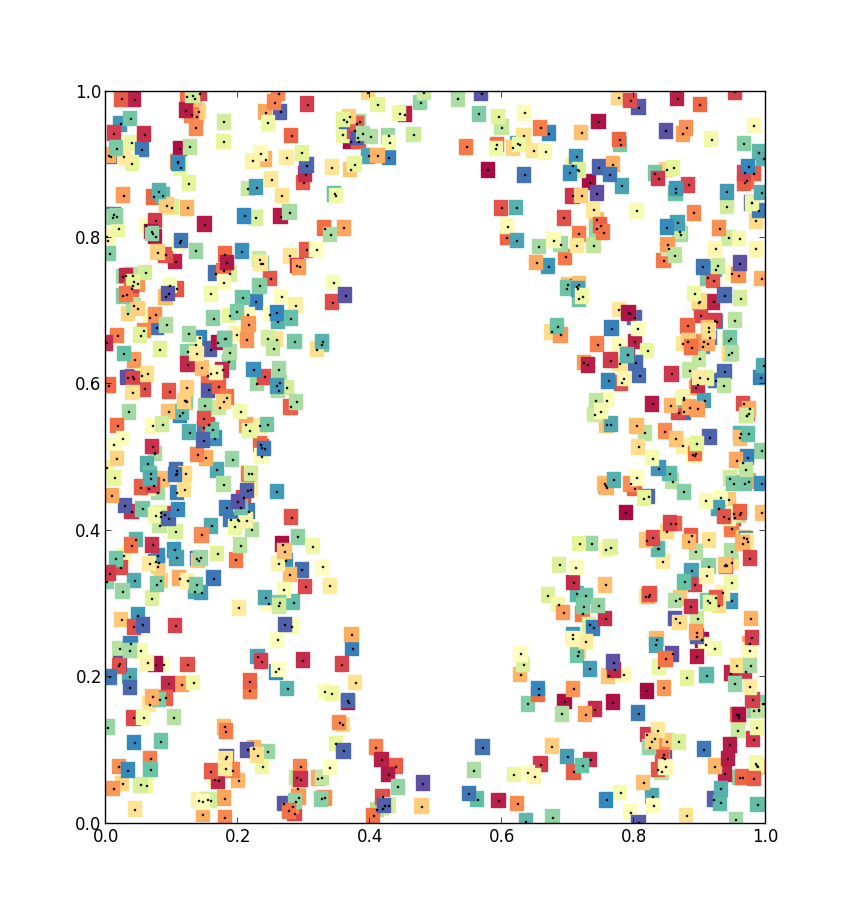
\includegraphics[width=0.4\textwidth]{random256}
  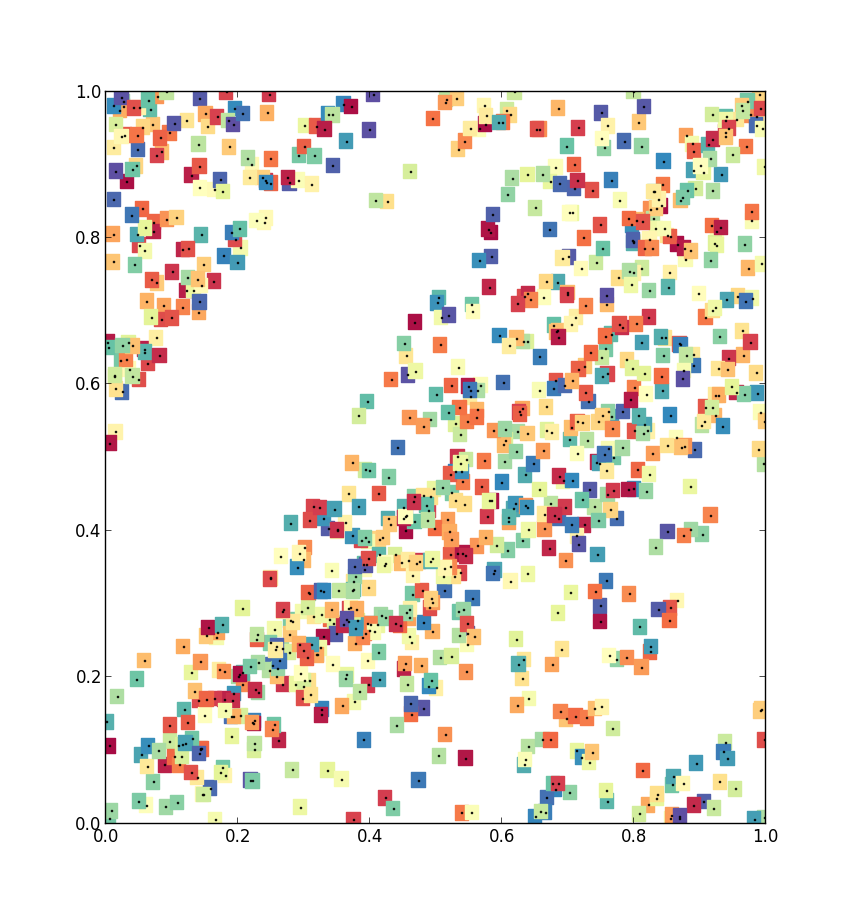
\includegraphics[width=0.4\textwidth]{random1280}
  \caption{Even after random iterations, a process that seem to create a chaos, orderly figures may suddenly emerge.}
  \label{fig:order}
\end{figure}
%
\begin{figure}[t]
  \centering
  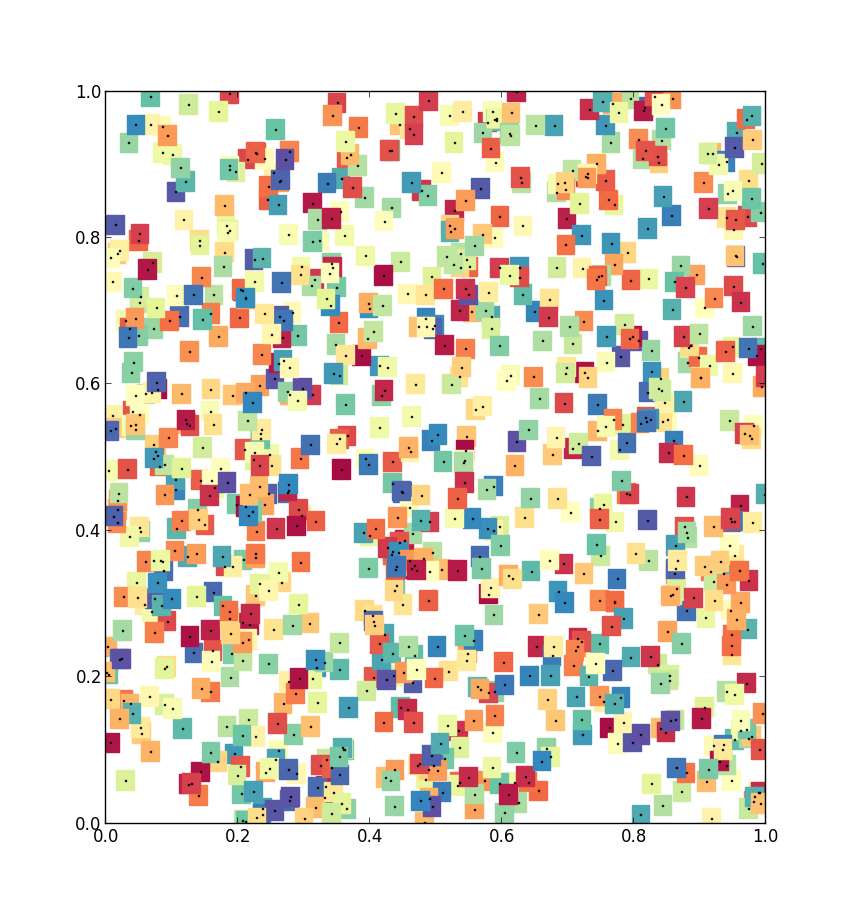
\includegraphics[width=0.6\textwidth]{chaotic_shape}
  \caption{Another example of a square of area 0.64 after 128 random iterations of the cat map and kick map.
  Most of time, random iterations will create a disorderly figure.
  }
  \label{fig:chaotic}
\end{figure}

The random iteration of the cat map and kick map is a good way to generate random shapes.

\subsection{Computing the Boundary}
As we saw in the previous sections, a shape generated by chaotic maps applied to a square is not necessarily a single piece (Fig.~\ref{fig:chaotic}).
We need an algorithm that computes the boundary of a given shape in order to run heat equation simulations for these shapes.
The \textit{boundary fill algorithm} 

For each point with the target color, if p has a neighbor with the non-target color, then it is on the boundary.

Use boundary fill to check the integrity of a shape.
Randomly pick a point -> Boundary fill from the init point -> If total colored area $\geq$ A (the area started with) throw away that sample (the flooded leaked outside the shape); if the shape is a bit smaller than $A$, it's ok (ok if new area $\geq 3/4 A$).


\section{The Optimal Wall}

\section{The Heat Equation}
This will be a two step problem.  First I'll solve heat for the batter with unknown boundary conditions on the sides, then I'll solve it for the pan to derive those boundary conditions.

\subsection{Part 1} 
Consider a rectangular mass of batter flush with the first octant and having width $W$, height $H$, and depth $l$.  Let the width of the baking pan be $D$.  Let $K$ be the conduction constant for brownie batter.  Let $T_i$ be the initial temperature of the batter and let $T_b$ be the baking temperature.  Let $f$ be the heat function for the brownie pan, let $r = (x,y,z)$ and $s = x+D,y+D,z+D$.   We wish to find the a function $T$ satisfying
\[\partial{T}{t} = K \nabla^2 T\]
subject to the initial condition
\[T(x,y,z,0) = T_i\]
and boundary conditions \begin{align*}
T(0,y,z,t) = T(W,y,z,t) &= f(s,t)\\
T(x,0,z,t) = T(x,L,z,t) &= f(s,t)\\
T(x,y,0,t) &= f(s,t)\\
T(x,y,H,t) &= T_b \end{align*}
where $s$ modifies the coordinates on the term to the left.
To simplify the following computations, define
\[u(r,t) = T(r,t) - f(s,t)\]
The equation becomes 
\[\frac{\partial u}{\partial t} K \nabla^2 u\]
with initial condition
\[u(r,0) = T_i - f(s,t)\]
and boundary conditions \begin{align*}
T(0,y,z,t) = T(W,y,z,t) &= 0\\
T(x,0,z,t) = T(x,L,z,t) &= 0\\
T(x,y,0,t) &= 0\\
T(x,y,H,t) &= T_b\end{align*}
We get away with not subtracting from the last equation because the top of the batter is not exposed to the pan.\\
\\
Approaching this by separation of variables, suppose
\[u(r,t) = XYZG\]
where $X,Y,Z$, and $G$ are functions of $x,y,z$, and $t$.  We find that \begin{align*}
u_t &= XYZG'\\
u_{xx} &= X''YZG\\
u_{yy} &= XY''ZG\\
u_{zz} &= XYZ''G \end{align*}
Plugging these into the heat equation and dividing by $KXYZG$, we find \begin{align*}
XYZG' &= K(X''YZG +XyY'ZG + XYZ''G)\\
\implies \frac{G'}{KG}  = \frac{X''}{X} + \frac{Y''}{Y} + \frac{Z''}{Z} \end{align*}
note that the left hand side of this equation is constant, so the right must be as well.  Introducing $\lambda^2$, we write
\[\frac{G'}{KG} = -\lambda^2 \hspace{15mm} \frac{X''}{X} + \frac{Y''}{Y} + \frac{Z''}{Z} = -\lambda^2\]
From the first equation, we immediately get the ODE
\[G'-G\lambda^2 = 0\]
For the other, let
\[\frac{X''}{X} = -\frac{Y''}{Y} - \frac{Z''}{Z} - \lambda^2 = -\mu^2\]
then 
\[\frac{Y''}{Y} = -\frac{Z''}{Z} - \lambda^2 + \mu^2 = -\nu^2\]
and
\[\frac{Z''}{Z} = - \lambda^2 + \mu^2 + \nu^2 = -\rho^2\]
\\
We can now derive the following equations: \begin{align*}
X''+ \mu^2 X &= 0\\
Y'' + \nu^2 Y &= 0\\
Z'' + \rho^2 Z &= 0 
\lambda^2 &= \mu^2 + \nu^2 + \rho^2
\intertext{and the one from before}
G'-G\lambda^2 = 0 \end{align*}
The general solution $G$ is $G = A e^{-\lambda^2 K t}$ for some constant $A$.  The general solution for $X'' + \mu^2 X = 0$ is 
\[X = c_1 \cos \mu x + c_2 \sin \mu x\]
Considering the boundary condition $X(0) = 0$, note that $c_1 = 0$.  Considering $X(W) = 0$, we must have $c_2 \sin \mu W = 0$.  Since $c_2=0$ is a trivial case, we focus on cases where $\sin \mu W = 0$.  This happens when $\mu W$ is an integer multiple of $\pi$.  We note therefore that
\[\mu_m = \frac{m \pi}{W}\]
for $m = 1,2, \dots$.  Substituting these findings into the equation for $X$, we find solutions
\[X_m(x) = \sin(\frac{m \pi x}{W})\]
the same method leads to a solution for $Y$:
\[Y_n(y) = \sin(\frac{n \pi y}{L})\]
for $n = 1,2,\dots$.\\
For $Z$, the boundary conditions are $Z(0) = 0$ and $Z(H) = T_b$ so we let
\[Z = \gamma_l e^{\rho_l z} + \delta_l e^{-\rho_l z}\]
the boundary condition $Z(0) = 0$ gives us $\gamma_l = -\delta_l$.  Choosing $\gamma_l = \frac{1}{2}$ we find
\[Z_l(z) = \sinh \rho_l z\]
the separated solution for $u$ is thus
\[u_{mnl}(r,t) = A_{mnl} \sin(\mu_m x) \sin (\nu_n y) \sinh (\rho_l z) e^{-\lambda^2_{mnl}Kt}\]
with
\[\lambda_{mnl}^2 = \mu_m^2 + \nu_n^2 + \rho_l^2 = \left(\frac{m \pi}{W}\right)^2 + \left(\frac{n \pi}{L} \right)^2 + \left(\frac{l \pi}{H}\right)^2\]
for $m,n,l = 1,2 \dots$\\
We can also form a linear superposition:
\[u(r,t) = \ssum_{m=1}^\infty \ssum_{n=1}^\infty \ssum_{l=1}^\infty A_{mnl} \sin(\mu_m x) \sin (\nu_n y) \sinh (\rho_l z) e^{-\lambda^2_{mnl}Kt}\]
with constants $A_{mnl}$.  This general solution satisfies the boundary conditions on all sides except the top.  To determine the values of the constants $A_{mnl}$, note the initial condition
\[u(r,0) = T_i - f(s,0)\]
we find
\[T_i - f(s,0) = \ssum_{m,=1}^\infty \ssum_{n=1}^\infty \ssum_{l=1}^\infty A_{mnl} \sin(\mu_m x) \sin (\nu_n y) \sinh (\rho_l z) \]
Let 
\[b_m(y,z) = \ssum_{n=1}^\infty \ssum_{l=1}^\infty A_{mnl} \sin (\nu_n y) \sinh (\rho_l z)\]
and consider that 
\[T_i - f(s,0) = \ssum_{m=1}^\infty b_m(y,z) \sin (\mu_m x)\]
we multiply both sides by $\sin (\mu_k x)$ and integrate, interchanging the integral and sum on the left: \begin{align*}
\int_0^W (T_i - f(s,0)) \sin(\mu_k x) dx &= \ssum_{m=1}^\infty \int_0^W b_m(y,z) \sin(\mu_m x) \sin (\mu_k x) dx
\intertext{Take note that on the right hand side, the sines are orthogonal unless $k = m$, leaving}
\int_0^W (T_i - f(s,0)) \sin(\mu_m x) dx &= \int_0^W b_m(y,z) \sin(\mu_m x) \sin (\mu_k x)
&= \frac{b_m(y,z) W}{2}\\
\end{align*}
and so we have 
\[b_m(y,z) = \frac{2}{W} \int_0^W (T_i - f(s,0)) \sin(\mu_m x) dx\]
the same technique will produce the analogous
\[c_n(x,z) = \frac{2}{L} \int_0^L (T_i - f(s,0)) \sin(\mu_n y) dy\]
for the opposite side. In the vertical direction, we let
\[d_l(x,y) = \ssum_{m=1}^\infty \ssum_{n=1}^\infty \sin(\mu_m x) \sin (\nu n y)\]
and so \begin{align*}
T_i - f(s,0) &= \ssum_{l=1}^\infty d_l(x,y) \sinh (\rho_l z)\\
&= \ssum_{l=1}^\infty d_l(x,y) \dfrac{e^{\rho_l z} - e^{-\rho_l z}}{2}\\
&= \frac{1}{2} \ssum_{l=1}^\infty d_l(x,y) (e^{\rho_l z} - e^{-\rho_l z})\\
2(T_i - f(s,0)) &= \ssum_{l=1}^\infty d_l (x,y) e^{\rho_l z} - \ssum_{l=1}^\infty d_l(x,y) e^{-\rho_l z} \end{align*}
let 
\[\delta(r) = \ssum_{l=1}^\infty d_l(x,y) e^{\rho_l z}\]
and 
\[\gamma(r) = \ssum_{l=1}^\infty d_l(x,y) e^{-\rho_l z}\]
Then
\[2(T_i - f(s,0)) = \delta(r) - \gamma(r)\]
and by fourier series,
\[d_n = \frac{2}{H} \int_0^H \delta(r) e^{-\rho_l z} dz = \frac{2}{H} \int_0^H \gamma(r) e^{\rho_l z} dz\]

\subsection{Part 2}
We used the method of finite differences to model the diffusion of heat through the batter and pan.  We started by building a two dimensional model for a vertical cross section of a rectangular pan.  Let $U^t$ and $C$ be arrays of dimension $M \times N$.  Let $c_a$,$c_p$ and $c_b$ be the thermal conductivity constants of air, the pan material, and brownie batter.  Let $T_i$ and $T_b$ stand for initial batter temperature and baking temperature, let $\delta s = \frac{1}{N}$, and let $w$ be the thickness of the pan material in units.\\
\\
From a schematic perspective, $U^t_{i,j}$ will hold the temperature of point $(i,j)$ at time $t$ and $C_{i,j}$ will hold the corresponding thermal conductivity constant.  For an illustrative example of initial conditions, consider the $6 \times 6$ case with $w = 1$:
\[U^0 = \begin{pmatrix} T_b&T_b&T_b&T_b&T_b&T_b\\
					T_b&T_i &T_i&T_i&T_i&T_b\\
					T_b&T_i &T_i&T_i&T_i&T_b\\
					T_b&T_i &T_i&T_i&T_i&T_b\\
					T_b&T_i &T_i&T_i&T_i&T_b\\
					T_b&T_b&T_b&T_b&T_b&T_b \end{pmatrix} \hspace{20mm}
  C = \begin{pmatrix} c_a&c_a&c_a&c_a&c_a&c_a\\
				   c_a &c_p &c_b&c_b&c_p&c_a\\
				    c_a &c_p &c_b&c_b&c_p&c_a\\
  				 c_a &c_p &c_b&c_b&c_p&c_a\\
				 c_a &c_p &c_p&c_p&c_p&c_a\\
				c_a&c_a&c_a&c_a&c_a&c_a \end{pmatrix} \]		
To track the evolution of $U$ through time, we define the following partial derivatives for points $(i,j,k)$, with time-coordinate $q$: \begin{align*}
u_t &\approx \dfrac{u_{i,j}^{q+1} - u_{i,j}^q}{\Delta t}\\
u_{xx} &\approx \dfrac{u_{i+1,j}^q - 2u^q{i,j} + u_{i-1,j}^q}{(\Delta s)^2}\\
u_{yy} &\approx \dfrac{u_{i,j+1}^q - 2u_{i,j}^q + u_{i,j-1}^q}{(\Delta s)^2} \end{align*}
Given these, the heat equation
\[u_t = c (u_{xx} + u_{yy})\]
becomes
\[\dfrac{u_{i,j}^{q+1} - u_{i,j}^q}{\Delta t} = c  \left(\dfrac{u_{i+1,j}^q - 2u_{i,j}^q + u_{i-1,j}^q}{(\Delta s)^2} + \dfrac{u_{i,j+1}^q - 2u_{i,j}^q + u_{i,j-1}^q}{(\Delta s)^2}\right)\]
from which we can derive
\[u_{i,j}^{q+1} = u_{i,j}^q + c \cdot \frac{\Delta t}{(\Delta s)^2} \left(u_{i+1,j}^q + u_{i-1,j}^q - 4u_{i,j}^q + u_{i,j+1}^q + u_{i,j-1}^q \right)\]
$\Delta t$, the length of a timestep, can be chosen arbitrarily but must obey the relation
\[\Delta t \leq \frac{(\Delta s)^2}{2c}\]
for $c = c_a,c_p,c_b$ for a stable solution.\\
\\
Using values $m = 8, n=8, T_b = 176, T_i = 26, \Delta t = 1/50000, c_a = .024$, and $c_b = .017$, , we varied the conduction coefficient for the pan to determine the best pan material for even heating around the edges.  We first compared glass ($c_p = 1.05$) to a much less conductive material ($c_p = 0.05$) and aluminum ($c_p = 215$) and reached the following states after 20000 timesteps:
\[c_p = 0.05: \begin{pmatrix} 176&176&176&176&176&176\\
						176&115.87&63.98&63.98&115.87&176\\
						176&93.66&38.64&38.64&93.66&176\\
						176&95.14&42.41&42.41&95.14&176\\
						176&122.43&95.38&95.38&122.43&176\\
					        176&176&176&176&176&176 \end{pmatrix}\] 
\[c_p = 1.05: \begin{pmatrix} 176&176&176&176&176&176\\
						176&136.34&71.99&71.99&136.34&176\\
						176&122.18&49.61&49.61&122.18&176\\
						176&127.61&60.92&60.92&127.61&176\\
						176&152.16&129.42&129.42&152.56&176\\
					        176&176&176&176&176&176 \end{pmatrix}\]
\[c_p = 215: \begin{pmatrix} 176&176&176&176&176&176\\
						176&136.85&72.48&72.48&136.85&176\\
						176&122.91&50.37&50.37&122.91&176\\
						176&128.41&62.09&62.09&128.41&176\\
						176&152.67&130.25&130.25&152.66&176\\
					        176&176&176&176&176&176 \end{pmatrix}\]
Noting the corner values of $122.43, 152.16$, and $152.67$, we were struck by the lack of difference between glass and aluminum.  We repeated the test on glass and aluminum with $14 \times 14$ arrays, and reached the following states in the lower left corners after 50,000 timesteps:

We concluded from this that, assuming a minimal level of conductivity (on par with glass), an increase in conductivity does little to increase or allay heat buildup around the edges of the pan.\\
\\
Our next step was to design an analogous scheme for the three-dimensional problem.  Using the partial derivatives 
\end{enumerate}


\section{Testing and Results}
Model Testing and Sensitivity Analysis, including error analysis, etc.
\subsection{Strengths and Weaknesses}

Example of tabular environment (using booktab environment. from wikibooks) 

\begin{tabular}{llr}
\toprule
\multicolumn{2}{c}{Item} \\
\cmidrule(r){1-2}
Animal    & Description & Price (\$) \\
\midrule
Gnat      & per gram    & 13.65      \\
          & each        & 0.01       \\
Gnu       & stuffed     & 92.50      \\
Emu       & stuffed     & 33.33      \\
Armadillo & frozen      & 8.99       \\
\bottomrule
\end{tabular}

\section{Conclusion}
Need a connected component algorithm.
Flood-fill algorithm is an example of such an algorithm.

% The bibliography is in a separate file
\renewcommand{\bibname}{References}
\bibliographystyle{plainnat}
\nocite{*}
\bibliography{mcmbib}

\end{document}
